\input{/home/d1r3ct/.config/preamble.tex}

\title{Programming Paradigms, Answers to lecture notes}
\begin{document}
\maketitle


\textit{Lecture 8.}

When you're calling multiple functions, let's say $A, B, C$, how do stack
frames get placed on the stack? How it behaves when you call a function
multiple times, where it places the allocated stack frame?

\textit{Lecture 13.}
\begin{enumerate}
    \item If we're redefine a function prototype and call let's say ``strlen"
    function with 2 parameters, the linker phase is still going to allocate the
    space for all the parameters, but the actual function implementation will only
    know about the first one.

    \textit{Answer:}

    \item Why dereferencing of null pointer causes segfaults? What ``segments" are there?

        \textit{Answer:}
        Because it points to the 0th address and this is not of the known
        segments. Known segments in RAM are:
        \begin{itemize}
            \item stack
            \item heap
            \item code segments
            \item data segment
        \end{itemize}

        \begin{figure}[h]
            \centering
            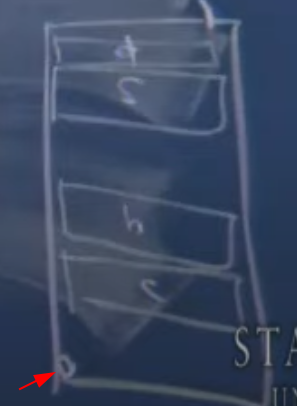
\includegraphics[width=0.3\linewidth]{ram-segments.png}
            \caption{Null address in RAM}%
            \label{fig:ram_segments}
        \end{figure}


    \item Bus errors, explain why does integers start at a multiple of 4?
        Shorts at a multiple of 2? What might cause a bus error?

        \textit{Answer:}
        It's when you dereference an address that resides in one of 4 known
        segments, but it's an odd address and you dereference a short, that is
        always stored at even (divisible by two) address.

        \begin{lstlisting}
void *vp = malloc();
*(short *) vp = 7; // Bus error when address not multiple of 2.
*(int *) vp = 52; // Bus error when address not multiple of 4.
        \end{lstlisting}
\end{enumerate}

\textit{Lecture 14.}
\begin{itemize}
    \item How can we do an argument overload in a function like printf?

    \textit{Answer:}
    It's done by putting the data the stack and then using the control string
        to unpack it. That string is a roadmap for the rest of the parameters.
    \begin{figure}[h]
        \centering
        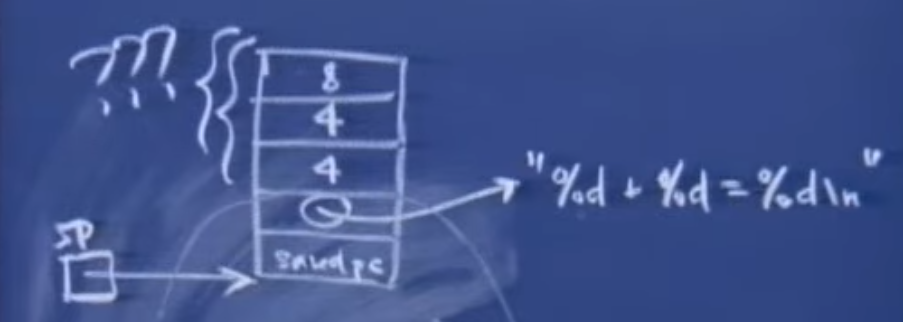
\includegraphics[width=0.8\linewidth]{argument-overloading.png}
        \caption{Argument overloading}%
        \label{fig:arg_overloading}
    \end{figure}
\end{itemize}

\end{document}
